%******************************************************************************************************
%*********************************** First Chapter ****************************************************
%******************************************************************************************************

\chapter{Introduction}  %Title of the First Chapter
\label{intro}

% **************************** Define Graphics Path **************************
\ifpdf
    \graphicspath{{Chapter1/Figs/Raster/}{Chapter1/Figs/PDF/}{Chapter1/Figs/}}
\else
    \graphicspath{{Chapter1/Figs/Vector/}{Chapter1/Figs/}}
\fi


%******************************************************************************************************
%******************************************************************************************************
\section{An Introduction to Unmanned Aerial Vehicles} 
\label{intro:UAVs}

The term Unmanned Aerial Vehicle (UAV) can be used to describe any form of aircraft that does not require a pilot on board. This term includes aircraft that are controlled remotely, autonomous vehicles capable of navigating themselves, and any aircraft that are a combination of the two. Other terms that may be familiar are ``drone'' and Unmanned Aerial System (UAS), which can be used interchangeably with UAV within the context of this project. 

UAVs come in a wide range of form factors but can be split into two main classes; fixed-wing UAVs and rotary wing UAVs. Fixed-wing UAVs are generally only capable of horizontal take-off and landing (HTOL), whilst rotary wing UAVs generally employ vertical take-off and landing (VTOL). There are, however, other forms of UAV which incorporate features of both main classes; for example, quadplane UAVS use rotary wing rotors to allow VTOL, but do the main bulk of their flying with forward facing rotors much like a fixed-wing UAV. Across these categories are a very wide range of UAV platforms, from hobbyist quadcopters to military attack vehicles, and many many others in between. %TODO images?  
Although the range of UAV form factors and their uses is vast, the vast majority are suitable for candidates for complete autonomous flight control, as shall be described in Section %TODO reference where we talk about adding hardware modules 
 
Although there were a large number of suitable candidates for the following work, it was decided that this project would be aimed at the control of strictly fixed-wing UAVs for the purposes of aerial photography. For that reason, we shall not discuss any other style of UAV. %TODO 

%******************************************************************************************************
%******************************************************************************************************
\section{UAVs for Aerial Photography} 
\label{intro:photography}

The first recorded use of aerial photography was in 1858 by a French balloonist and photographer known as ``Nadar'' at a height of 80 metres using a tethered hot air balloon. %TODO ref aerial photography history
Since then aerial photography has of course massively progressed, both in terms of the aerial vehicles in use and the cameras available. As such, it is now an activity that can be partaken in by both organisations, companies, and individuals alike, for a range of purposes. For example, aerial photography of course plays a very large role in intelligence gathering by government agencies and militaries, but can also be a hobby for otherwise earth-bound photography enthusiasts. 

Different applications will require different equipment and styles of photography; a hobbyist may want a wide panorama, whilst a mapping application will require a consistent vertical camera angle. The use of aerial photography for mapping or measurement is known as aerial photogrammetry, and will be the chosen field of interest for this project. Aerial photogrammetry is a specific subset of aerial photography in that it not only requires the capturing of images, but additional information about where the image was captured. For this project, we are looking at the use of aerial photogrammetry to create an image of the land below our UAV, either for mapping or general surveying purposes. In order to be able to do this, we need to be able to capture a set of images, and know the location of the UAV when the images were captured, to allow the images to be stitched together into one larger image of the ground beneath. In this scenario we can typically use GPS co-ordinates and a pre-planned imaging path to define which images relate to which areas of the ground below. %TODO refernce photogrammetry definition?


This project will primarily focus on the mapping of land beneath the UAV, and as such we need to define a specified flightpath over the chosen area. There are a number of typical flightpaths for surveying or mapping land, two forms are lawnmower pattern paths and spiral pattern paths. Fig. \ref{fig:simplelawnmower} shows the general form of a lawnmower pattern, and Fig. \ref{fig:simplespiral} shows us the general form of a spiral pattern.

\begin{figure}[htbp!] 
\centering    
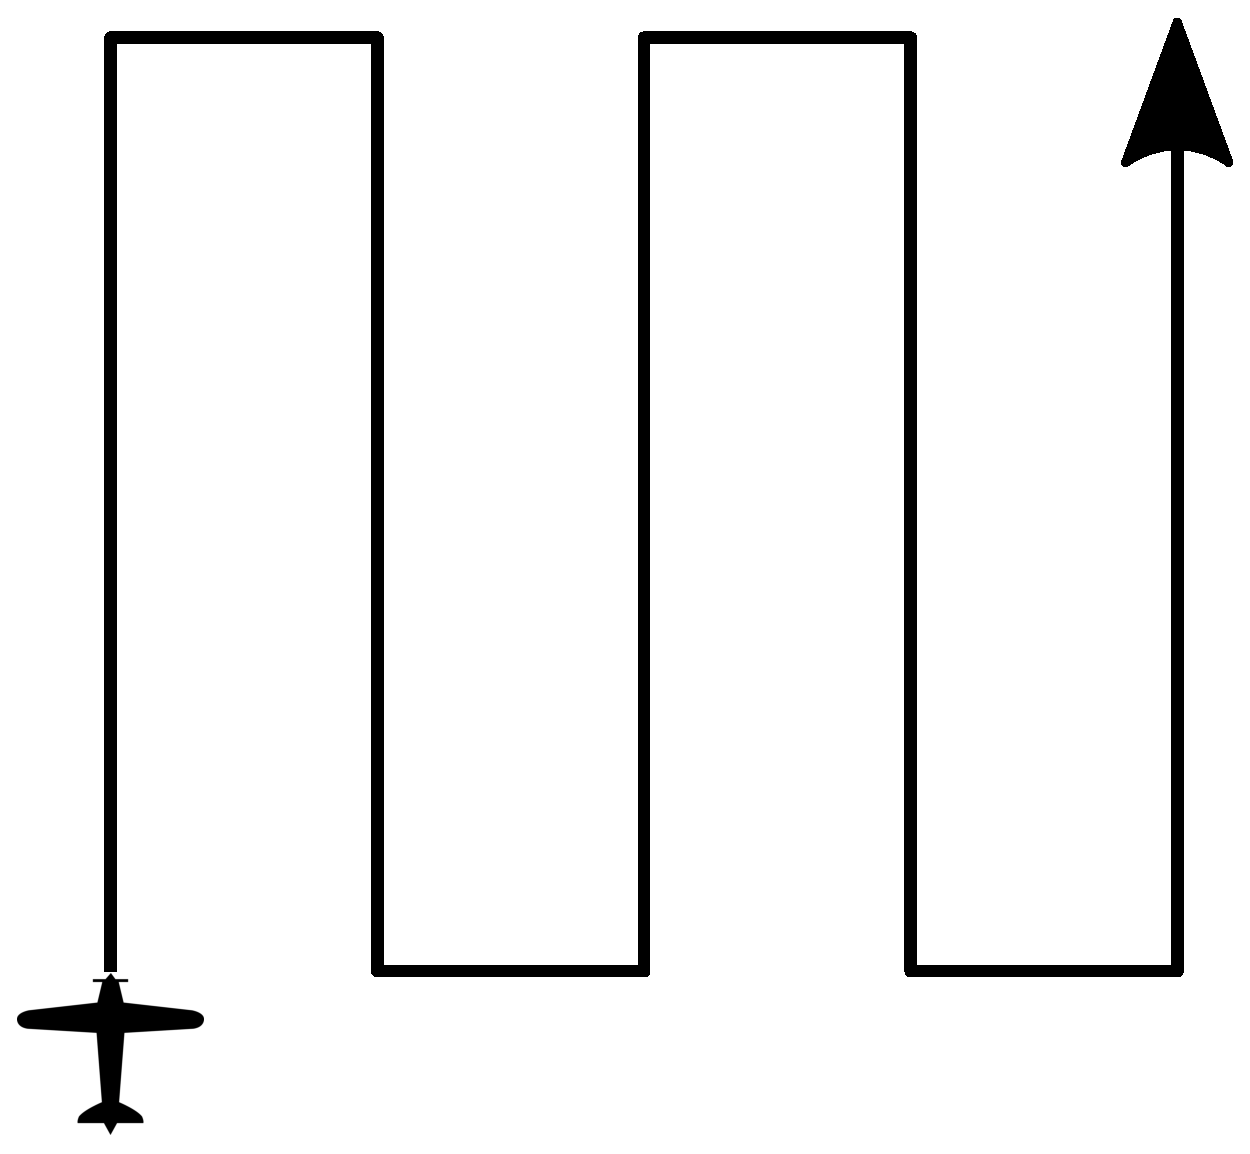
\includegraphics[width=0.5\textheight]{SimpleLawnmower}
\caption[Simple Lawnmower Pattern]{The general form of a lawnmower pattern aerial imaging run}
\label{fig:simplelawnmower}
\end{figure}

\begin{figure}[htbp!] 
\centering    
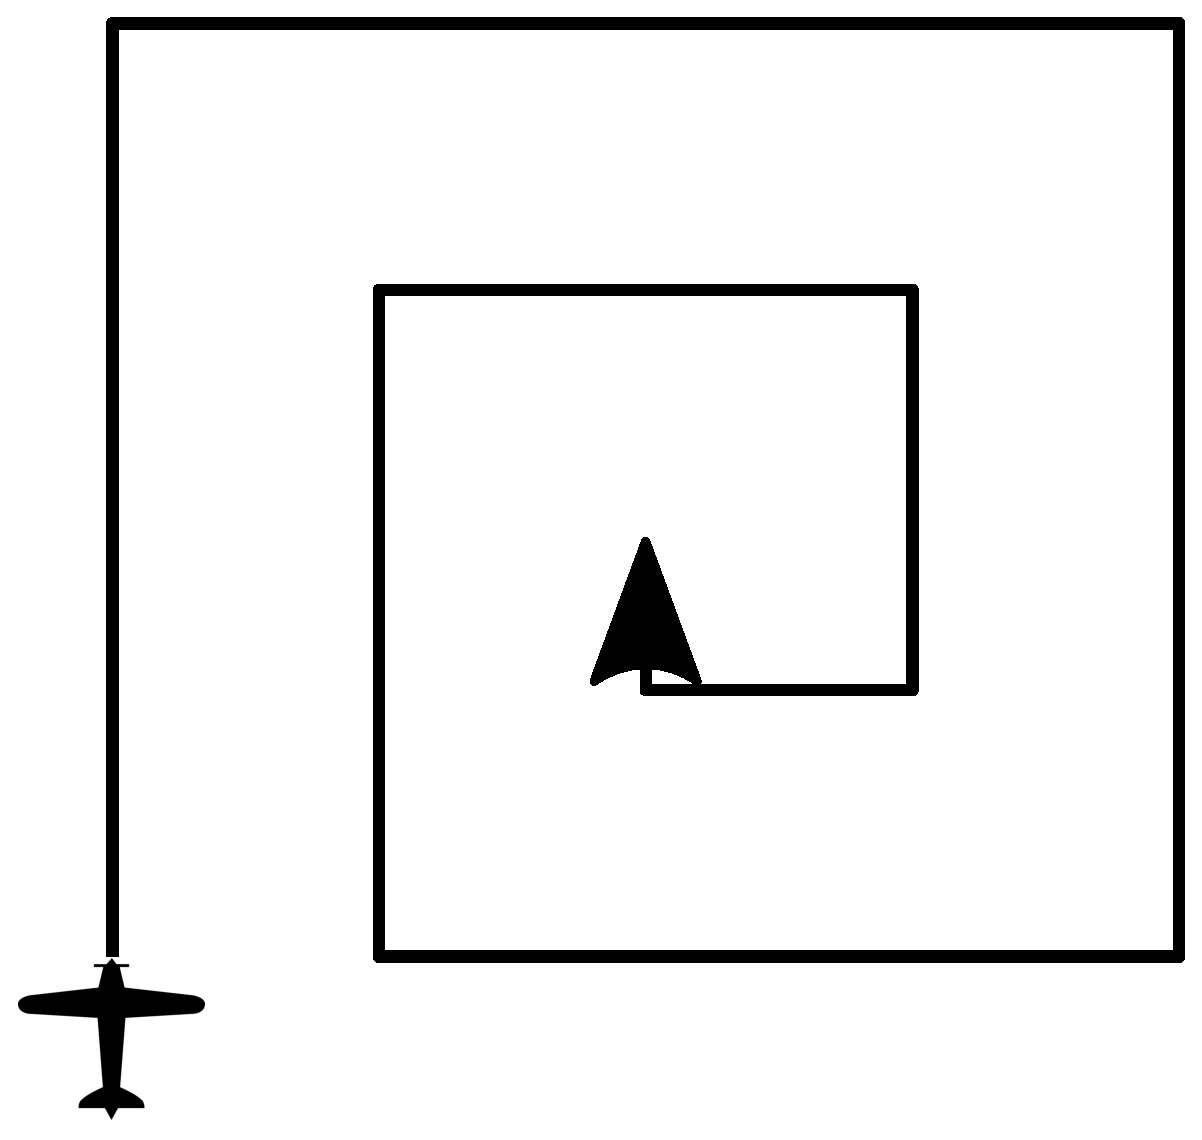
\includegraphics[width=0.5\textheight]{SimpleSpiral}
\caption[Simple Spiral Pattern]{The general form of a spiral pattern aerial imaging run}
\label{fig:simplespiral}
\end{figure}

Using these patterns, we can define what shall be referred to henceforth as ``imaging paths'' or ``imaging runs''. These are the sections of the flightpath for which we are capturing images of the ground below, and as such we very much care about the position and orientation of the UAV whilst following these paths. For the lawnmower pattern the imaging paths are the vertical sections of the path seen in Fig. \ref{fig:simplelawnmower}, whereas for the spiral path all sections of the flight plan are considered imaging paths. 

As the lawnmower pattern does not require the horizontal sections of the path in Fig. \ref{fig:simplelawnmower} to be used for capturing images, we are not particularly concerned with how we fly between the imaging paths. Knowing this, we can specify our flightpath in terms of simply our imaging paths, as can be seen in Fig. \ref{fig:imaginglawnmower}

\begin{figure}[htbp!] 
\centering    
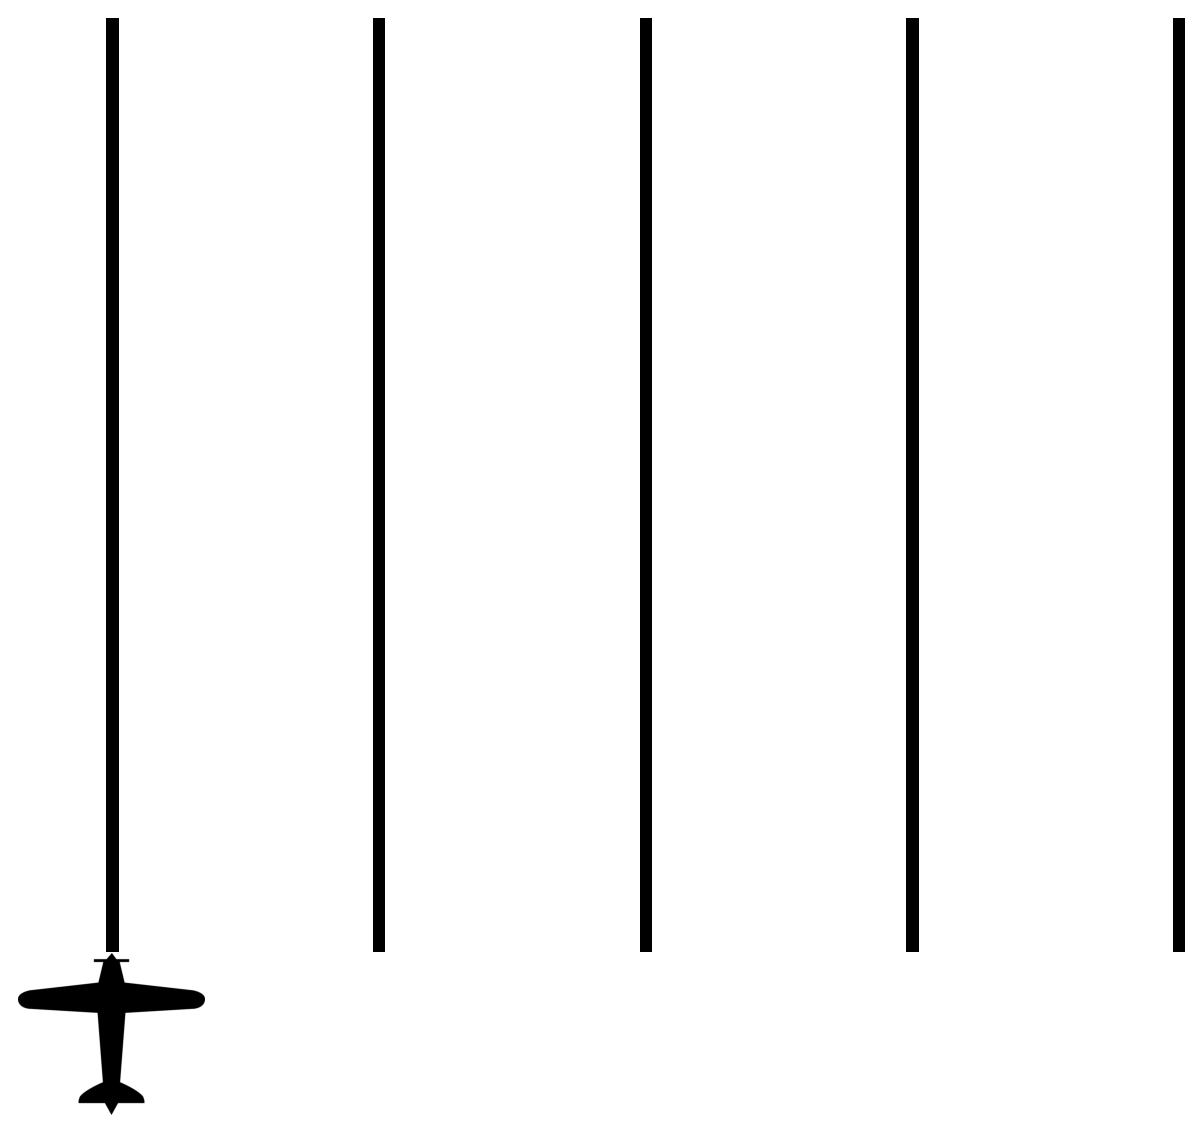
\includegraphics[width=0.5\textheight]{ImagingLawnmower}
\caption[Imaging Lawnmower Pattern]{A version of the lawnmower pattern, using only imaging paths}
\label{fig:imaginglawnmower}
\end{figure}

As the imaging paths shown in Fig. \ref{fig:imaginglawnmower} are separate of one another, it is possible to complete each imaging path in any order and in either direction. This does however require the user to plan accordingly and to record location data accurately so as to be able to stitch together the resulting photographs correctly. One of the resulting patterns that we can create from this is called the ``Zamboni pattern'', named after the route a Zamboni machine takes around an ice rink to smooth out the ice. %TODO remove zamboni nonsense?

The required flightpath will have to be calculated based on a number of factors including:
\begin{itemize}
	\item The size of the area we are wishing to photograph
	\item Changes in ground elevation over the chosen area
	\item The operational range of the UAV based on battery life or fuel amount
	\item The desired resolution of the resulting images - we must fly lower for higher detail images
	\item The distance between imaging paths will be a function of the desired flying height and the angle of the lens on the camera
	\item The path to follow between the imaging paths will be a function of the turning performance of the UAV
	\item Environmental factors such as wind during the flight
\end{itemize}

These factors shall be considered and discussed later in this report where relevant, and have been used to inform decisions throughout the work of this project.

%******************************************************************************************************
%******************************************************************************************************
\section{ArduPilot and ArduPlane} 
\label{intro:arduplane}

ArduPilot is an open-source suite of autopilot products aimed at hobbyists and professionals alike. ArduPilot includes the ArduPlane, ArduCopter, and ArduRover autopilots, each aimed at aeroplane style UAVS, helicopter and multirotor UAVS, and ground based rover UAVs respectively. As previously mentioned, this project is aimed at fixed-wing aeroplane UAVs, and as such this report is looking at the ArduPlane product. 

ArduPilot has been around since late 2009 and was originally designed to operate using the Arduino development ecosystem.

\subsection{JSBSim}
\label{intro:jsbsim}

JSBSim is the simulator packaged with ArduPlane for testing purposes

\subsection{MissionPlanner and APM Planner}
\label{intro:planner}


%******************************************************************************************************
%******************************************************************************************************
\section{Autopilot Hardware} 
\label{intro:hardware}



